% Generated by build_manuscript.py from 05_results.md
\section{5 Results and discussion}\label{results-and-discussion}

\subsection{5.1 Prediction quality under matched acquisition caps}\label{prediction-quality-under-matched-acquisition-caps}

Task-driven feedback produced lower observed errors than several fixed acquisition rules under the common 25\% cap. The main policy achieved a pooled MAE of 44.286 MPa, RMSE of 58.517 MPa and R² of 0.659 on the 50 validation specimens. Geometry-spread achieved 46.910 MPa MAE, giving a paired improvement of 2.624 MPa with a 95\% exploratory interval of {[}−0.488,5.925{]} MPa. The actual acquired fraction for the main policy averaged 0.247437 and ranged from 0.234492 to 0.249999. The comparison is therefore at a matched cap, with small specimen-dependent differences in the completed native-pixel fractions.

Across the entire acquisition range, the main policy had a six-domain-equal A of 45.110 MPa, compared with 47.311 MPa for geometry-spread. The lower area indicates that its advantage was not confined to the terminal estimate. However, area and terminal quality capture different properties: Random had a slightly lower endpoint MAE than geometry-spread but a higher A. Inspecting only the final state would miss this difference in the quality supplied during acquisition. Figure 2 retains the observed stepwise MAE paths, including reversals, and Supplementary Table S2 reports all five common caps with their actual acquisition ranges.

{ % do not increment counter
\begin{center}\begin{minipage}{\linewidth}\small
\begin{tabular}{@{}
  >{\raggedright\arraybackslash}p{(\linewidth - 10\tabcolsep) * \real{0.3750}}
  >{\raggedleft\arraybackslash}p{(\linewidth - 10\tabcolsep) * \real{0.1250}}
  >{\raggedleft\arraybackslash}p{(\linewidth - 10\tabcolsep) * \real{0.1250}}
  >{\raggedleft\arraybackslash}p{(\linewidth - 10\tabcolsep) * \real{0.1250}}
  >{\raggedleft\arraybackslash}p{(\linewidth - 10\tabcolsep) * \real{0.1250}}
  >{\raggedleft\arraybackslash}p{(\linewidth - 10\tabcolsep) * \real{0.1250}}@{}}
\toprule\noalign{}
\begin{minipage}[b]{\linewidth}\raggedright
Acquisition policy
\end{minipage} & \begin{minipage}[b]{\linewidth}\raggedleft
A (MPa)
\end{minipage} & \begin{minipage}[b]{\linewidth}\raggedleft
Early A (MPa)
\end{minipage} & \begin{minipage}[b]{\linewidth}\raggedleft
MAE at cap (MPa)
\end{minipage} & \begin{minipage}[b]{\linewidth}\raggedleft
RMSE at cap (MPa)
\end{minipage} & \begin{minipage}[b]{\linewidth}\raggedleft
R² at cap
\end{minipage} \\
\midrule\noalign{}



Center-first & 48.475 & 51.821 & 48.027 & 65.223 & 0.577 \\
Geometry-spread & 47.311 & 51.880 & 46.910 & 62.278 & 0.614 \\
Serpentine & 48.911 & 52.170 & 48.013 & 63.041 & 0.605 \\
Random & 49.594 & 54.117 & 46.886 & 61.941 & 0.618 \\
Learned-static & 47.977 & 52.946 & 46.993 & 62.168 & 0.616 \\
No-VLM spatial feedback & 43.597 & 48.771 & 42.385 & 56.534 & 0.682 \\
VLM mean feedback & 45.263 & 50.390 & 43.611 & 59.012 & 0.654 \\
VLM spatial feedback (main) & 45.110 & 49.642 & 44.286 & 58.517 & 0.659 \\
VLM spatial open-loop & 46.501 & 51.048 & 44.822 & 59.663 & 0.646 \\
Complete input, fraction 1.0 & --- & --- & 41.690 & 53.944 & 0.711 \\
\bottomrule\end{tabular}
\end{minipage}\end{center}
}

\textbf{Table 3. Common-predictor comparison.} Partial policies use cap 0.25; the complete-input row is a separate cost-1.0 reference. A integrates over 0--0.25 and early A over 0--0.0625, each normalized by its own interval. Areas weight domains equally; endpoint measures pool physical specimens after repeat-loss averaging. All values are selected-validation estimates, with n=50 physical specimens. Actual fraction ranges and full paired results are provided in the supplementary source tables.

\begin{figure}
\centering
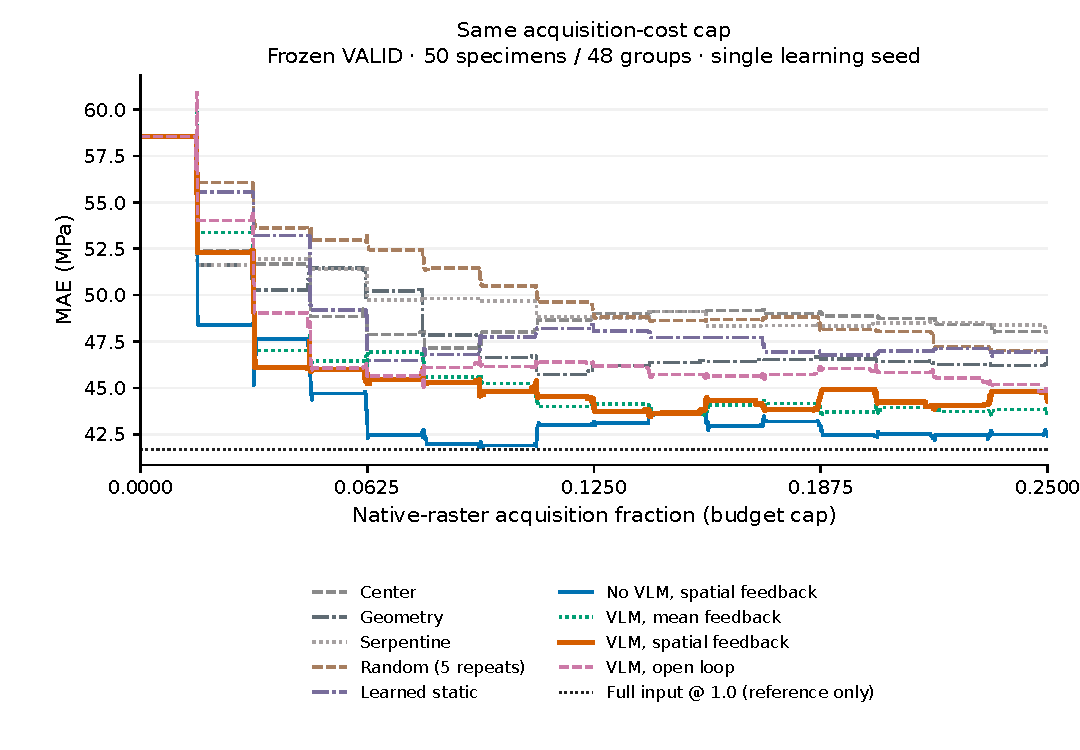
\includegraphics[width=1\linewidth,height=\textheight,keepaspectratio,alt={MAE along the recorded acquisition range. Curves are held current-state values on the shared event grid, with no smoothing. The complete-input horizontal reference represents quality measured only at cost 1.0.}]{figures/Fig2_mae.pdf}
\caption{MAE along the recorded acquisition range. Curves are held current-state values on the shared event grid, with no smoothing. The complete-input horizontal reference represents quality measured only at cost 1.0.}
\end{figure}

\subsection{5.2 From a shared order to evidence-dependent acquisition}\label{from-a-shared-order-to-evidence-dependent-acquisition}

The three policies spanning a shared ranking, specimen-conditioned open-loop choice and internal feedback had progressively lower area estimates: 47.977, 46.501 and 45.110 MPa. This sequence connects the experiment to the intended engineering distinction. Learned-static offers one order for every specimen. Open-loop can use surface variation to allocate observations differently, while feedback can revise its allocation after seeing internal content. Their performance pattern is consistent with useful specimen dependence, followed by further improvement when current acquired evidence participates in the next decision.

The main policy improved on open-loop by 1.391 MPa in A and 0.536 MPa in endpoint MAE. The area direction favoured feedback in five of the six domains. The comparison therefore links feedback to a lower observed trajectory loss over much of this cohort, while the interval in Table 4 retains uncertainty about the difference. These adjacent contrasts do not identify percentages of total improvement caused by individual modules: policies were separately trained, used different initializations and visited different states. Their value is to show the consequences of distinct decision-information arrangements under the same assessment model.

{ % do not increment counter
\begin{center}\begin{minipage}{\linewidth}\small
\begin{tabular}{@{}
  >{\raggedright\arraybackslash}p{(\linewidth - 6\tabcolsep) * \real{0.2308}}
  >{\raggedright\arraybackslash}p{(\linewidth - 6\tabcolsep) * \real{0.2308}}
  >{\raggedleft\arraybackslash}p{(\linewidth - 6\tabcolsep) * \real{0.3077}}
  >{\raggedright\arraybackslash}p{(\linewidth - 6\tabcolsep) * \real{0.2308}}@{}}
\toprule\noalign{}
\begin{minipage}[b]{\linewidth}\raggedright
Contrast, control minus main
\end{minipage} & \begin{minipage}[b]{\linewidth}\raggedright
Measure
\end{minipage} & \begin{minipage}[b]{\linewidth}\raggedleft
Difference (MPa)
\end{minipage} & \begin{minipage}[b]{\linewidth}\raggedright
95\% exploratory interval (MPa)
\end{minipage} \\
\midrule\noalign{}



Geometry-spread versus main & A & 2.200 & {[}−0.787,5.033{]} \\
Open-loop versus feedback & A & 1.391 & {[}−0.683,3.406{]} \\
No-VLM versus VLM & Early A & −0.872 & {[}−4.870,3.255{]} \\
Mean versus spatial feedback & A & 0.152 & {[}−2.186,2.425{]} \\
\bottomrule\end{tabular}
\end{minipage}\end{center}
}

\textbf{Table 4. Component-related comparisons.} Positive values favour the main policy for the stated measure. All four intervals contain zero. Intervals use the existing paired within-domain capture-group bootstrap and are conditional on selected validation checkpoints. Supplementary Figure S4 displays these contrasts; the VLM contrast uses early A rather than full-range A.

The no-VLM feedback policy obtained lower full-range A and endpoint MAE than the main policy, at 43.597 and 42.385 MPa, respectively. Its surface descriptors were still present, so this result concerns the additional VLM prior rather than the utility of surface information as a whole. Spatial interaction likewise provided a mixed comparison with mean feedback: the main actor's area was lower by 0.152 MPa and its RMSE by 0.495 MPa, but its endpoint MAE was higher by 0.675 MPa. These results support keeping the components conceptually distinct instead of treating architectural complexity as evidence of a uniform performance gain.

\subsection{5.3 When acquired evidence contributes to prediction quality}\label{when-acquired-evidence-contributes-to-prediction-quality}

The largest positive timing difference between feedback and open-loop acquisition occurred after the initial internal observations had become available. Main-minus-open-loop contributions across the four completion stages were +0.415, +1.296, −0.223 and −0.097 MPa. Their net sum corresponds to the main policy's 1.391 MPa lower error area. The second stage, spanning completion fractions above 0.0625 and up to 0.125, provided the largest positive difference. Thus, the observed trajectory difference cannot be summarized solely as selecting a better starting region.

The common predictor gives this comparison a specific interpretation. Each acquired subset changes the evidence supplied to the same regression mapping, and the completion time determines how long that updated estimate enters the area objective. Contributions assigned to the second stage are weighted over the remaining interval to B; the 1.296 MPa difference is not a local integral reduction confined to that stage. The main policy's absolute stage contributions were 11.031, 0.960, −0.091 and 0.038 MPa. Subtracting their sum from the common domain-equal initial error of 57.049 MPa gives A=45.110 MPa. This initial error differs from the pooled initial MAE of 58.551 MPa because the two estimands weight domains differently.

The timing pattern also distinguishes feedback from broad spatial coverage and a learned shared order. Geometry-spread obtained first- and second-stage contributions of 7.143 and 2.672 MPa; its smaller first-stage value was partly offset in the second stage. Learned-static obtained 9.729 MPa in the first stage, followed by −1.058 MPa in the second. Against open-loop, the main policy's second-stage contribution was positive while the control's was negative. This pattern is consistent with useful evidence-dependent allocation once initial internal information is available. The separately trained policies nevertheless differ in initialization and visited states, so the decomposition accounts for observed prediction changes rather than assigning a causal share to feedback.

\begin{figure}
\centering
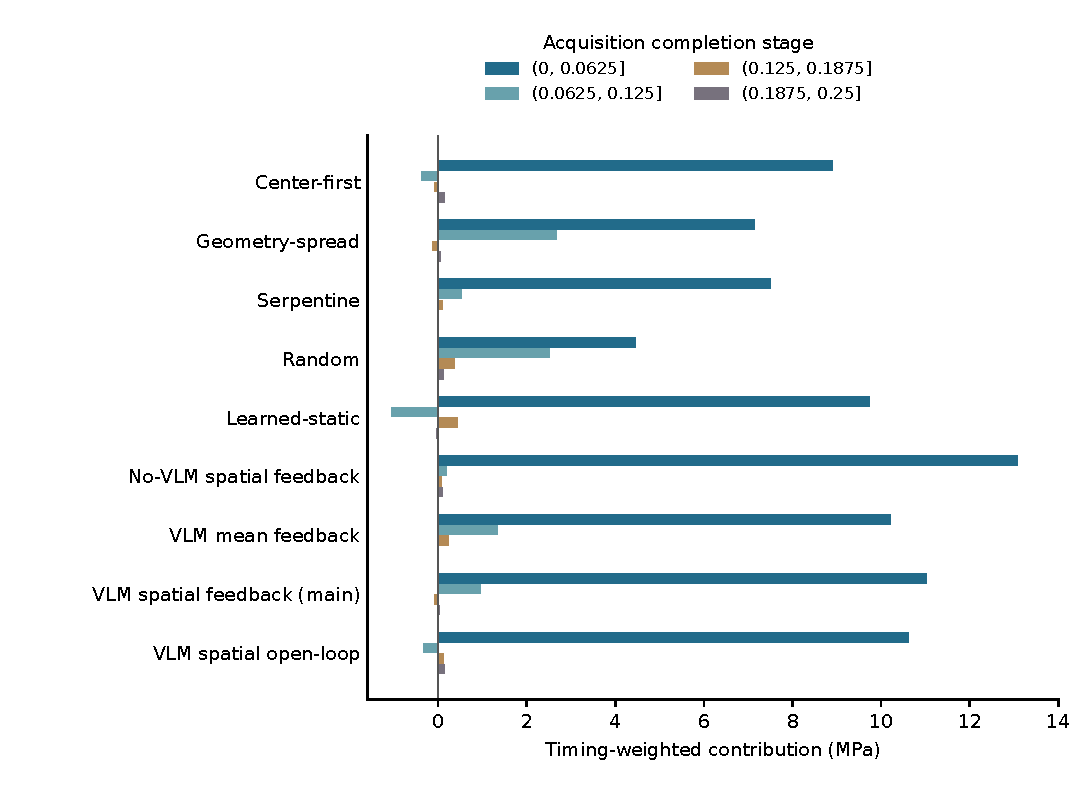
\includegraphics[width=1\linewidth,height=\textheight,keepaspectratio,alt={Timing-weighted error contributions grouped by acquisition completion stage. All nine methods and negative values are retained. Episode sums are averaged over repeats within specimen, within domain and equally across six domains, with 50 physical specimens. Contributions affect the remaining budget interval after completion; they are not stage-local error integrals.}]{figures/Fig4_timing.pdf}
\caption{Timing-weighted error contributions grouped by acquisition completion stage. All nine methods and negative values are retained. Episode sums are averaged over repeats within specimen, within domain and equally across six domains, with 50 physical specimens. Contributions affect the remaining budget interval after completion; they are not stage-local error integrals.}
\end{figure}

Later observations qualified the earlier improvement. The final two main-versus-open-loop differences were negative, and 381 of the main policy's 793 acquisitions increased individual absolute error. Revealing a descriptor can move a finite regressor's estimate away from the measured strength, even within a sequence with lower overall area. Retaining these signed changes makes the accounting compatible with the reversals in the quality curves. Useful state-dependent acquisition therefore concerns the resulting evidence sequence, rather than guaranteed error reduction after every action.

Figure 4 follows the existing c8-16 case after one and eight acquisitions, showing how the measured set and actual next action change as evidence accumulates. The first proposal was narrower than the ordinary legal set for 45 of 50 main-policy specimens; subsequent decisions used the expanded legal set and updated state. These panels illustrate that progression without changing the original observed content. The same three fixed cases remain in the supplement, including the higher-error q24-48 case and their prediction trajectories. Case images document executed choices; the timing comparison above summarizes their cohort-level prediction consequences.

\begin{figure}
\centering
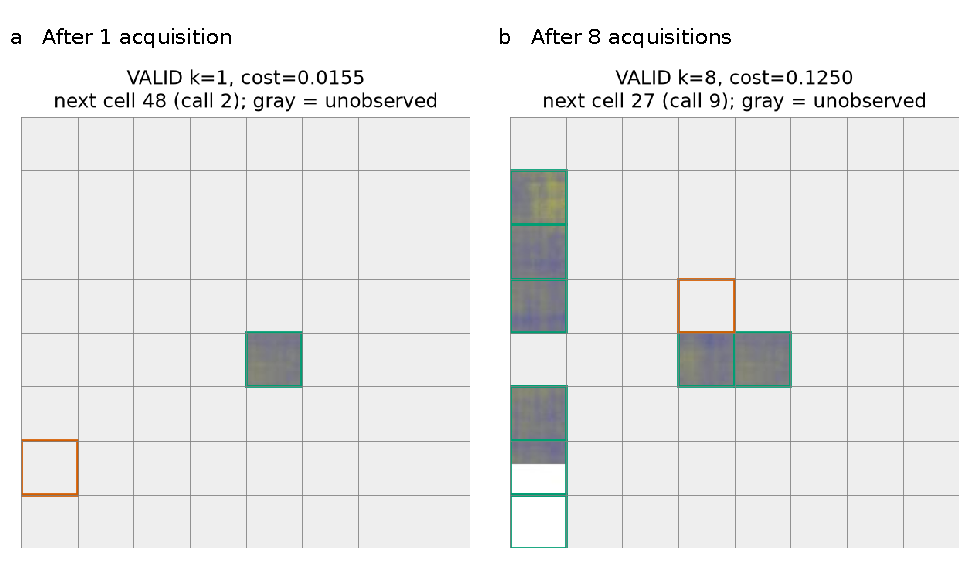
\includegraphics[width=1\linewidth,height=\textheight,keepaspectratio,alt={Acquisition progression for the preselected c8-16 specimen after one and eight acquisitions, ordered left to right. Both panels preserve the original native-cost annotations, next-cell identifier and observed/unobserved colors; grey cells remain unobserved. Panels show acquisition steps, not a matched-cost performance comparison. Source imagery: Hasebe et al., version-1 dataset, CC BY 4.0; the registered overlays are assembled unchanged.}]{figures/Fig4_case_process.pdf}
\caption{Acquisition progression for the preselected c8-16 specimen after one and eight acquisitions, ordered left to right. Both panels preserve the original native-cost annotations, next-cell identifier and observed/unobserved colors; grey cells remain unobserved. Panels show acquisition steps, not a matched-cost performance comparison. Source imagery: Hasebe et al., version-1 dataset, CC BY 4.0; the registered overlays are assembled unchanged.}
\end{figure}

\subsection{5.4 Acquisition requirements at matched empirical quality}\label{acquisition-requirements-at-matched-empirical-quality}

An acquisition advantage depends on the target quality and the comparator. At q=46.909917 MPa, the geometry-spread endpoint MAE used as one of the complete anchor set, the main policy first met the target at cap 0.0625 on the five-point grid. Geometry-spread first met it at 0.125, giving a 50\% reduction in the earliest supported cap. Learned-static also first met it at 0.0625, giving zero reduction relative to that comparator. Using geometry-spread's nominal 0.25 endpoint as its required cost would overstate the reduction, because that method had already reached the same empirical quality earlier.

The finer event grid resolves earlier crossings but also reveals their instability. For the same target, the earliest main, geometry and static caps were 0.031388, 0.093426 and 0.062407, respectively. These correspond to reductions of 66.40\% and 49.70\% against geometry and static on that grid. At the main policy's crossing, its actual mean fraction was 0.030861 and MAE was 46.507051 MPa; its curve subsequently rose above the target. We retain this event-grid result in the supplementary analysis, separately from the primary 50\% and 0\% comparisons, because grid resolution and first-passage reversals materially change its interpretation.

Figure 5 presents the full main-grid target range rather than a single favourable threshold. Supplementary tables retain all integer targets and source-labelled anchors on both grids, including unreached targets and negative or undefined ratios. This representation answers a practical descriptive question: at what supported cap did each population curve first achieve a specified quality? It does not supply an individual stopping certificate. An operational stopping policy would need information available without knowing the specimen's true CAI strength, and the present first-passage calculation does not provide that capability.

\begin{figure}
\centering
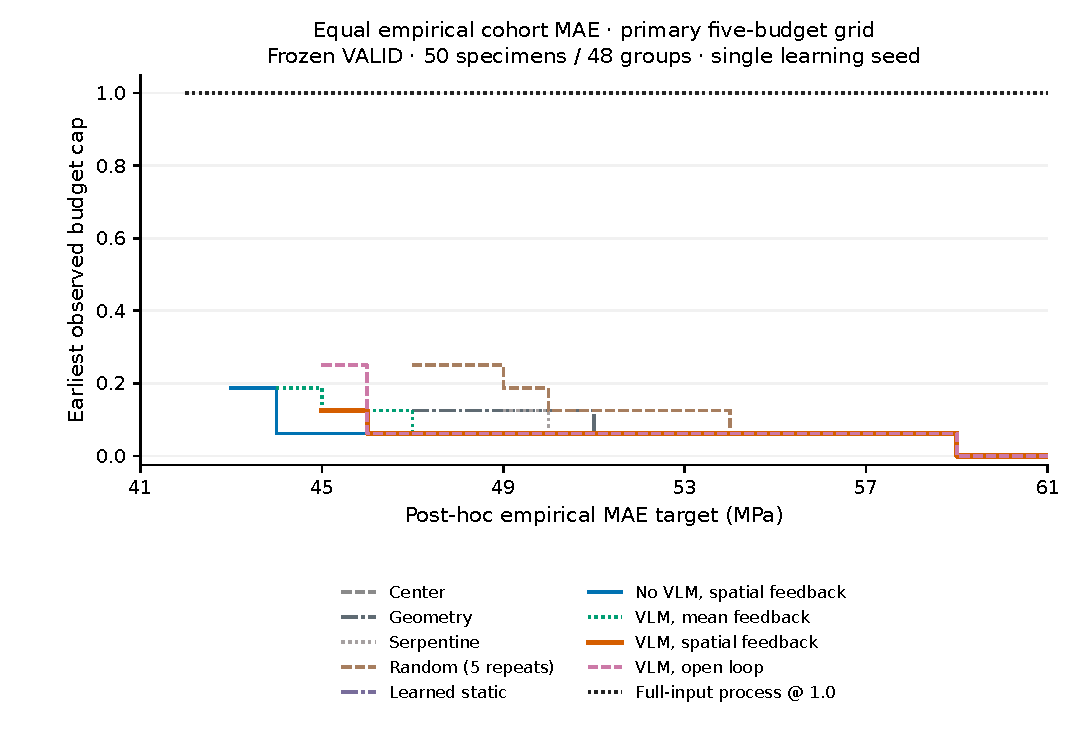
\includegraphics[width=1\linewidth,height=\textheight,keepaspectratio,alt={Earliest supported cap at each empirical MAE target on the primary five-cap grid. Missing points denote unreached quality; the finer event-grid results remain separate. The curves summarize cohort-level first passages, not a specimen stopping policy.}]{figures/Fig6_quality.pdf}
\caption{Earliest supported cap at each empirical MAE target on the primary five-cap grid. Missing points denote unreached quality; the finer event-grid results remain separate. The curves summarize cohort-level first passages, not a specimen stopping policy.}
\end{figure}

\subsection{5.5 Full-information trade-off and engineering interpretation}\label{full-information-trade-off-and-engineering-interpretation}

The common predictor with complete internal and surface input achieved 41.690 MPa MAE, 53.944 MPa RMSE and R²=0.711. The main policy at the 25\% cap therefore retained a 2.596 MPa MAE gap to complete input. None of the nine partial-acquisition policies reached the complete-input MAE anywhere in either observed grid. The full-input point helps locate the quality cost of partial observation under this predictor, but does not define an optimal industrial reference or a missing trajectory between fractions 0.25 and 1.0.

The engineering contribution is the explicit coupling between an assessment objective and the organization of acquired information. A policy can be compared at a shared cap, through its complete observed error trajectory, and at a shared empirical quality target. The timing contrast explains why area and terminal MAE need not agree: an observation changes the error over the remaining acquisition interval, not just at the endpoint. Together with target-dependent first passages, this connects sequential information acquisition to the image-based assessment objective. The contribution is a way to organize and evaluate observations according to that objective, rather than a new regression architecture or a universal acquisition-reduction percentage.

Domain-level results further bound the comparison. Against geometry-spread, the main policy's area difference favoured it in three domains and favoured the control in three. Against open-loop, five domain differences favoured feedback. This heterogeneity is compatible with acquisition decisions depending on specimen evidence, but it also leaves room for differences in predictor quality, source imaging and the distribution of specimens across domains. The reported data do not determine a material-specific causal explanation. The supplementary domain table preserves these directions without treating the six domains as six independent replications of the entire learning experiment.

The current evidence supports an offline image-acquisition method and a quality--acquisition analysis on a selected validation cohort. Physical deployment remains a separate question because native image pixels omit probe travel, coupling, setup and measurement latency; a 25\% image fraction cannot be translated directly into a 75\% time saving. A single policy-seed panel and validation-based selection also limit inference about reproducibility and transport to new specimens. The results establish the observed quality--acquisition relationships within that replay protocol; their transfer to independent specimens and physical inspection operations remains to be evaluated.
